%% This is file `elsarticle-template-1-num.tex',
%%
%% Copyright 2009 Elsevier Ltd
%%
%% This file is part of the 'Elsarticle Bundle'.
%% ---------------------------------------------
%%
%% It may be distributed under the conditions of the LaTeX Project Public
%% License, either version 1.2 of this license or (at your option) any
%% later version.  The latest version of this license is in
%%    http://www.latex-project.org/lppl.txt
%% and version 1.2 or later is part of all distributions of LaTeX
%% version 1999/12/01 or later.
%%
%% The list of all files belonging to the 'Elsarticle Bundle' is
%% given in the file `manifest.txt'.
%%
%% Template article for Elsevier's document class `elsarticle'
%% with numbered style bibliographic references
%%
%% $Id: elsarticle-template-1-num.tex 149 2009-10-08 05:01:15Z rishi $
%% $URL: http://lenova.river-valley.com/svn/elsbst/trunk/elsarticle-template-1-num.tex $
%%
%\documentclass[preprint,12pt]{elsarticle}

%% Use the option review to obtain double line spacing
% \documentclass[preprint,review,12pt]{elsarticle}

%% Use the options 1p,twocolumn; 3p; 3p,twocolumn; 5p; or 5p,twocolumn
%% for a journal layout:
%% \documentclass[final,1p,times]{elsarticle}
%% \documentclass[final,1p,times,twocolumn]{elsarticle}
%% \documentclass[final,3p,times]{elsarticle}
 \documentclass[final,3p,times,twocolumn]{elsarticle}
%% \documentclass[final,5p,times]{elsarticle}
%% \documentclass[final,5p,times,twocolumn]{elsarticle}

%% if you use PostScript figures in your article
%% use the graphics package for simple commands
%% \usepackage{graphics}
%% or use the graphicx package for more complicated commands
\usepackage{graphicx}
\usepackage{caption}
\usepackage{subcaption}
\usepackage{xurl}
%% or use the epsfig package if you prefer to use the old commands
%% \usepackage{epsfig}

%% The amssymb package provides various useful mathematical symbols
\usepackage{amssymb}
%% The amsthm package provides extended theorem environments
%% \usepackage{amsthm}


%% The lineno packages adds line numbers. Start line numbering with
%% \begin{linenumbers}, end it with \end{linenumbers}. Or switch it on
%% for the whole article with \linenumbers after \end{frontmatter}.
\usepackage{lineno}

%% natbib.sty is loaded by default. However, natbib options can be
%% provided with \biboptions{...} command. Following options are
%% valid:

%%   round  -  round parentheses are used (default)
%%   square -  square brackets are used   [option]
%%   curly  -  curly braces are used      {option}
%%   angle  -  angle brackets are used    <option>
%%   semicolon  -  multiple citations separated by semi-colon
%%   colon  - same as semicolon, an earlier confusion
%%   comma  -  separated by comma
%%   numbers-  selects numerical citations
%%   super  -  numerical citations as superscripts
%%   sort   -  sorts multiple citations according to order in ref. list
%%   sort&compress   -  like sort, but also compresses numerical citations
%%   compress - compresses without sorting
%%
%%\biboptions{authoryear}

\journal{KIV/VI - Information Visualization}

\begin{document}
    
\begin{frontmatter}
        
%% Title, authors and addresses

%% use the tnoteref command within \title for footnotes;
%% use the tnotetext command for the associated footnote;
%% use the fnref command within \author or \address for footnotes;
%% use the fntext command for the associated footnote;
%% use the corref command within \author for corresponding author footnotes;
%% use the cortext command for the associated footnote;
%% use the ead command for the email address,
%% and the form \ead[url] for the home page:
%%
%% \title{Title\tnoteref{label1}}
%% \tnotetext[label1]{}
%% \author{Name\corref{cor1}\fnref{label2}}
%% \ead{email address}
%% \ead[url]{home page}
%% \fntext[label2]{}
%% \cortext[cor1]{}
%% \address{Address\fnref{label3}}
%% \fntext[label3]{}
        
%%%% Article title to be placed here

%%% see http://mirrors.nic.cz/tex-archive/macros/latex/contrib/elsarticle/doc/elsdoc.pdf

\title{Multidimensional dynamic visualization of multiple stock prices time series}     
%% use optional labels to link authors explicitly to addresses:
%% \author[label1,label2]{<author name>}
%% \address[label1]{<address>}
%% \address[label2]{<address>}

\author[KIV]{Lukáš Runt\corref{corJK}}
\ead{lrunt@stundets.zcu.cz}

\cortext[corJK]{Corresponding author}

\address[KIV]{Student of Software and Information Systems, Department of Computer Science and Engineering, Faculty of Applied Sciences, University of West Bohemia, Pilsen, Czechia}

%%%% Abstract text to be placed here %%%%%%%%%%%%
\begin{abstract}

This work presents an interactive tool for the scalable analysis of high-frequency time series from financial markets. These markets generate massive amounts of granular data, including individual stocks and Exchange Traded Funds, where malicious activities like spoofing often hide within market noise. The primary research question is how to efficiently identify and visually isolate positively correlated time series among thousands of stocks within specific time windows. Building upon the interactive visual analytics work of Dominik Zappe, this research enhances user interaction and the visual encoding of data. Specifically, it introduces 2D and 3D multivariate line charts, alongside sparklines and horizon charts that spatially separate individual time series. To support correlation analysis, a correlation matrix, UMAP, and t-SNE projections have been integrated. Furthermore, the system contains filtering options for visual clarity and a sorting mechanism that groups highly correlated time series together. After evaluating alternative technologies like JavaScript and the ROOT framework to address performance constraints, the original Python and Plotly implementation was retained, as the alternatives did not outperform it. Application of the tool demonstrates that the visualization effectively displays correlated data from multiple analytical perspectives. Integrated filtering successfully removes irrelevant categories, allowing seamless orientation within large datasets. While detecting sophisticated market manipulation like spoofing requires future validation by financial domain experts, this tool significantly assists in identifying suspicious patterns. Ultimately, the framework provides an effective, scalable solution that enhances the overall comprehension and exploration of complex financial datasets.

\end{abstract}

\begin{keyword}
    %% keywords here, in the form: keyword \sep keyword
    Vizualization\sep Time series\sep Financial market
    %% MSC codes here, in the form: \MSC code \sep code
    %% or \MSC[2008] code \sep code (2000 is the default)
    
\end{keyword}

\end{frontmatter}

%%%%%%%%%%%%%%% End of first page %%%%%%%%%%%%%%%%%%%%%

%%
%% Start line numbering here if you want
%%
\linenumbers

\section{Introduction}

Modern financial markets operate at sub-millisecond speeds, generating enormous volumes of high-frequency data primarily recorded in Limit Order Books (LOB). While this granularity provides deep insights into market microstructure, it also creates an environment where malicious trading activities can be easily masked by market noise. One of the most disruptive forms of market manipulation is spoofing. In a typical spoofing strategy, a malicious actor places large, non-bona fide orders on one side of the order book to create a false illusion of buying or selling pressure. This artificially drives the stock price up or down. Once the price reaches a favorable level, the spoofer executes their actual intended trade on the opposite side of the market and abruptly cancels the initial deceptive orders. Identifying such fraudulent behavior is critical for maintaining market integrity, yet it remains computationally and analytically challenging \cite{Cartea2020}.

To effectively uncover these hidden manipulative behaviors, interactive visual analytics present a promising solution for exploring complex financial datasets. However, visualizing thousands of granular time series simultaneously introduces a significant visual challenge. Standard plotting techniques inevitably lead to severe overplotting, creating dense, unreadable visualizations commonly referred to as a "hairball" (see Figure \ref{fig:hairballs_side_by_side}). In such cluttered environments, identifying synchronized patterns or distinguishing meaningful signals from market noise becomes practically impossible. A methodology is therefore required that can untangle this visual complexity to capture the coordinated movements that would otherwise remain obscured.

\begin{figure*}[htbp]
    \centering
    \begin{subfigure}[b]{0.48\textwidth}
        \centering
        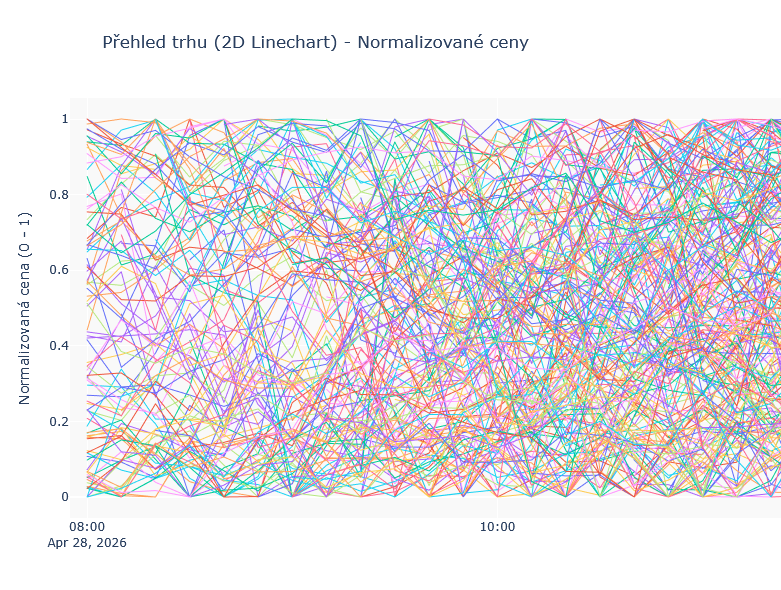
\includegraphics[width=\textwidth]{hairball_2.png}
        \caption{Standard 2D chart exhibiting severe visual clutter.}
        \label{fig:hairball_1}
    \end{subfigure}
    \hfill
    \begin{subfigure}[b]{0.48\textwidth}
        \centering
        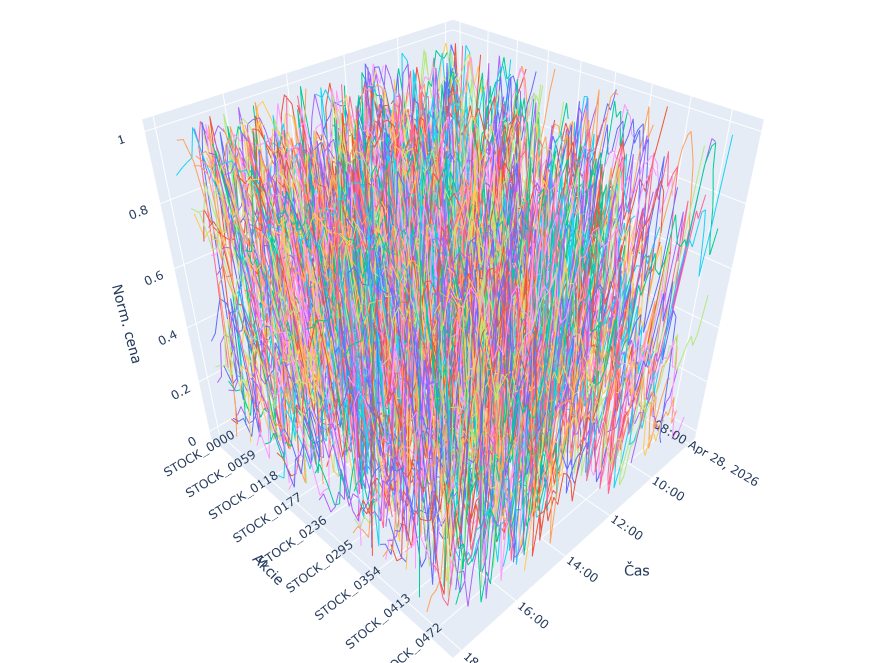
\includegraphics[width=\textwidth]{hairball.png}
        \caption{3D time-series plotting resulting in a dense hairball.}
        \label{fig:hairball_2}
    \end{subfigure}
    \caption{An example of visual clutter (the "hairball" effect) resulting from standard plotting of hunderds of high-frequency financial time series simultaneously. The high density of overlapping lines masks synchronized patterns and market noise, making analytical extraction impossible.}
    \label{fig:hairballs_side_by_side}
\end{figure*}

The purpose of this study is to address this gap by developing an interactive tool for the scalable analysis and visual isolation of positively correlated time series within specific time windows. Building upon the foundational interactive visual analytics work of Dominik Zappe, this research significantly enhances user interaction and the visual encoding of data to de-clutter the "hairball." By introducing spatially separated visualizations such as sparklines and horizon charts, alongside advanced dimensionality reduction techniques like UMAP and t-SNE, the system allows analysts to seamlessly filter, sort, and group highly correlated assets. Furthermore, by directly linking these macro-level correlational views to micro-level 2D and 3D LOB visualizations, the proposed approach empowers analysts to drill down and verify the specific deceptive order flows driving manipulated price movements.

\section{Related Work}\label{sec:relatedwork}

Financial data visualization generally falls into two distinct paradigms, namely interactive visual analytics tailored for web exploration and high performance computing frameworks designed for batch processing of massive datasets. This research positions itself at the intersection of these areas to bridge the gap between interactivity and computational scalability.

This study directly builds upon the foundational work of Dominik Zappe, who developed an interactive visual analytics tool specifically designed for the exploratory analysis of historical LOB data. Implemented within a modern web-centric Python ecosystem (utilizing Plotly, plotly-resampler, and Dash), Zappe’s architecture adopts a dual-view design to facilitate essential details-on-demand workflows. By integrating a macro-level Heatmap Matrix to aggregate metrics across multiple instruments with a micro-level multivariate Price Chart, this framework successfully enables analysts to detect temporal outliers and visually drill down into specific spoofing patterns \cite{Zappe2025}. 

hen researchers attempt to resolve this loss of detail by plotting raw 2D time series lines, the interface suffers from a strict theoretical limit. Displaying massive amounts of granular data across thousands of instruments inevitably generates a dense and unreadable visual clutter commonly referred to as a hairball. Consequently, standard interactive heatmaps or cluttered 2D line tools fail to scale effectively for granular exploratory workflows, necessitating advanced visual encoding and spatial separation techniques.

\subsection{3D Time Series Visualization}\label{sec_3D_plot}
To address the visual congestion inherent in displaying thousands of lines, existing literature examines the utility of projecting temporal data into three dimensional spaces. Bach et al. \cite{bach2014review} and Zhu et al. \cite{zhu2012visualizing} demonstrated that mapping time, distinct instruments, and prices onto three separate axes creates spatial trajectories that reveal parallel behaviors. This multilayered visualization style allows analysts to detect synchronized movements and high positive correlations across multiple assets simultaneously. However, while these historical studies prove that 3D projections successfully expose global market topologies, they frequently note that static 3D plots suffer from occlusion and perspective distortion, a limitation that necessitates advanced user interaction and filtering.

\subsection{Sparklines and Spatial Separation}\label{sec_sparklines}
To overcome the visual clutter inherent in shared space line graphs, researchers frequently employ spatially separated micro charts. Tufte \cite{tufte2006beautiful} introduced sparklines as data intense and design simple graphics that present historical trends without traditional axes or labels. In financial analytics, arranging these sparklines in a small multiples layout allows researchers to scan hundreds of asset profiles simultaneously to identify sudden spikes or structural breaks. However, Javed et al. \cite{javed2010graphical} empirically demonstrated that spatially separating multiple time series into individual canvases drastically diminishes vertical screen space. Consequently, while sparklines excel at providing rapid qualitative summaries and eliminating occlusion, their extreme vertical compression requires high cognitive effort for precise quantitative comparisons. This justifies the necessity of interactive environments where these compressed macro level views are seamlessly paired with detailed micro level charts.

\subsection{Horizon Charts for High Density Stacking}\label{sec_horizon}
To maximize screen space efficiency without sacrificing vertical resolution, researchers utilize layered visual encodings that support multi series scalability. Originally developed by Saito et al. \cite{saito2005two} and evaluated extensively by Heer et al. \cite{heer2009crowdsourcing}, horizon charts split a time series into multiple virtual bands, mirror negative values, and overlay them within a single baseline slot. This technique drastically reduces the required vertical space while preserving the ability to detect fine grained price movements across multiple instruments. Expanding upon this foundation, Javed et al. \cite{javed2010graphical} conducted empirical comparisons demonstrating that as the number of concurrent time series increases, horizon charts significantly outperform shared space line graphs in visual discrimination tasks. Their research confirms that while standard plotting rapidly degrades into visual clutter, the layered architecture of horizon charts maintains high reading accuracy even under extreme screen space constraints. Despite their capacity to completely eliminate line crossing and the hairball effect, these empirical studies concurrently warn that horizon charts demand a steeper learning curve for users compared to basic plotting, a factor that requires careful implementation and interactive support in high stress analytical environments.

\subsection{Correlation Visualization and Dimensionality Reduction}\label{sec_correlation}
To analyze dependencies across thousands of financial instruments, researchers rely on visual methods that map asset relationships into readable structures. Traditionally, a standard correlation matrix represents pairwise linear coefficients within a tabular grid. While a matrix provides exact mathematical values, empirical studies demonstrate that it scales quadratically with the number of assets, making macro pattern discovery virtually impossible when analyzing thousands of series simultaneously due to extreme visual clutter \cite{ghoniem2004readability}. To address this scalability limit, modern literature utilizes dimensionality reduction techniques to project complex correlation profiles into lower dimensional layouts. 

Algorithms such as t-SNE and UMAP compress the high dimensional behavior of multiple assets into two or three spatial coordinates where positively correlated instruments form distinct clusters \cite{shao2016visual}. Specifically, van der Maaten and Hinton \cite{vandermaaten2008visualizing} designed t-SNE to excel at preserving local neighborhoods and separating dense clusters, though subsequent research notes it often fails to maintain global market topologies and requires significant computational time. In contrast, McInnes et al. \cite{mcinnes2018umap} introduced UMAP, which preserves both local and global relationships more effectively while scaling efficiently to massive datasets. However, these projection methods compress raw information, which introduces a research gap regarding how these abstract spatial groups can be seamlessly linked back to actual high frequency price charts.

\section{Methods}\label{sec:methods}
This section outlines the methodology for analyzing thousands of high frequency financial time series. The workflow encompasses extracting Limit Order Book data, incorporating pre computed anomaly detection metrics, performing dimensionality reduction, and constructing a multi layered visual analytics interface equipped with advanced filtering capabilities.

\subsection{Data Source and Preprocessing}\label{sec:data}

The main data source consists of six transaction files capturing historical market activity from the Deutsche Börse. This data was originally downloaded via the A7 API during previous research. For the purposes of this study, the data is processed as raw, message-level event streams in a JSON format. These streams detail complete order flow transactions, including order additions, modifications, executions, and deletions. 

Preprocessing involved parsing these raw transaction messages and chronologically reconstructing the full state of the LOB for each point in time. For consistency and portability, the resulting order book snapshots were stored in a structured CSV format corresponding to the LOBSTER standard. This format represents 30 depth levels of bids and asks, including their respective prices and volumes.

\subsection{Visual Encoding and Interface Implementation}\label{sec_visual_encoding}
The frontend architecture features a dual layout designed to support exploratory workflows. The top section acts as a micro level verification tool, displaying raw high frequency order book dynamics. The bottom section provides a macro level overview utilizing multiple spatial separation techniques. A 2D multivariate line graph isolates pre filtered trajectories using high contrast color coding, while a 3D time series projection maps time, distinct instruments, and values onto separate axes. Both implementations feature a dynamic highlight mechanism, allowing users to visually emphasize specific trajectories against the dimmed surrounding data. 

To completely eliminate line crossing and enable high density stacking, two compressed visualization techniques were engineered. Sparklines were constructed utilizing a minimalistic vertical footprint and a hidden baseline to provide rapid qualitative summaries of individual asset trends. Finally, horizon charts were implemented by dividing the continuous time series into multiple virtual color bands, mirroring negative values, and overlaying them within a single baseline slot.

\subsection{Correlation Analysis and Dimensionality Reduction}\label{sec_correlation_analysis}
To systematically analyze market dependencies and structure the visual output, a mathematical correlation pipeline was integrated into the backend. Initially, a pairwise correlation matrix was computed to quantify linear relationships between all selected instruments over sliding time windows. Because a raw matrix becomes visually unreadable with massive datasets, dimensionality reduction algorithms were applied. Specifically, the high dimensional correlation profiles were passed into t-SNE and UMAP algorithms. 

To ensure stable structural groupings, key hyperparameters within these algorithms were systematically configured. The perplexity parameter within the t-SNE algorithm was carefully tuned to balance local and global neighborhood sizes, while the number of neighbors and minimum distance parameters for UMAP were adjusted to optimize the density and separation of the projected financial clusters. These algorithms compressed the complex relationships into two dimensional spatial coordinates, automatically grouping positively correlated assets into distinct analytical clusters. This resulting structural design fundamentally prepares the data for objective visual assessment.

\subsection{User Interaction, Filtering, Preprocessing and Correlation Sorting}\label{sec_sorting_methods}
To effectively navigate the large data volume and manage visual congestion within the macro level views, interactive filtering and data processing mechanisms were integrated into the interface. A categorical filtering system was engineered to allow analysts to isolate specific individual assets via a multi selection dropdown menu.

To support diverse analytical perspectives, a data transformation pipeline was implemented within the backend callback architecture. The system exposes three distinct preprocessing variants that users can dynamically toggle. The first variant preserves the raw aggregated values to maintain absolute market magnitudes. The second variant applies min max normalization to rescale all selected time series into a uniform zero to one range, enabling direct visual comparison across instruments with vastly different baseline scales. The third variant calculates the percentage change relative to the initial value captured at the beginning of the day, which isolates relative directional trends and volatility variations regardless of absolute price levels.

To structure the visual output logically, an automatic sorting pipeline was implemented within the backend callback structures. When a subset of assets is selected, the system dynamically computes a pairwise Pearson correlation matrix across the processed time series. This correlation matrix is subsequently transformed into a distance profile and processed using a hierarchical clustering algorithm with ward linkage. The algorithm computes an optimized leaf ordering that rearranges the underlying data arrays so that highly correlated assets with synchronized temporal behaviors are rendered adjacent to one another. Furthermore, the interface supports an alternative reference-based sorting mode, in which the user selects a single time series as a reference instrument. The backend then ranks all remaining assets by their Pearson correlation coefficient computed against this reference trajectory, rendering the most strongly correlated instruments at the top of the visual stack. This mode enables targeted identification of assets that most closely mirror a specific trajectory of interest. This architectural design fundamentally prepares the multi series datasets for objective visual assessment and localized pattern recognition.

\section{Results and Discussion}\label{sec:results}

The implementation of the proposed visual analytics architecture successfully addresses the challenge of identifying and verifying positive correlations among multiple high-frequency time series. By replacing the static heatmap with dynamic, multidimensional line visualizations, the system provides a more intuitive and scalable workflow for market anomaly detection. The analytical capabilities of the dashboard are demonstrated in the following figures.

\subsection{Evaluation of Analytical Framework ROOT}\label{sec:frameworks}
To address the massive data volume, the high performance ROOT framework was initially tested. However, empirical evaluation revealed it lacked the required interactivity and was poorly optimized for web based details on demand workflows. Consequently, development reverted to the Python ecosystem, utilizing libraries such as Plotly and Dash, and overcoming memory constraints through dynamic data aggregation.

\begin{figure}[h]
\centering
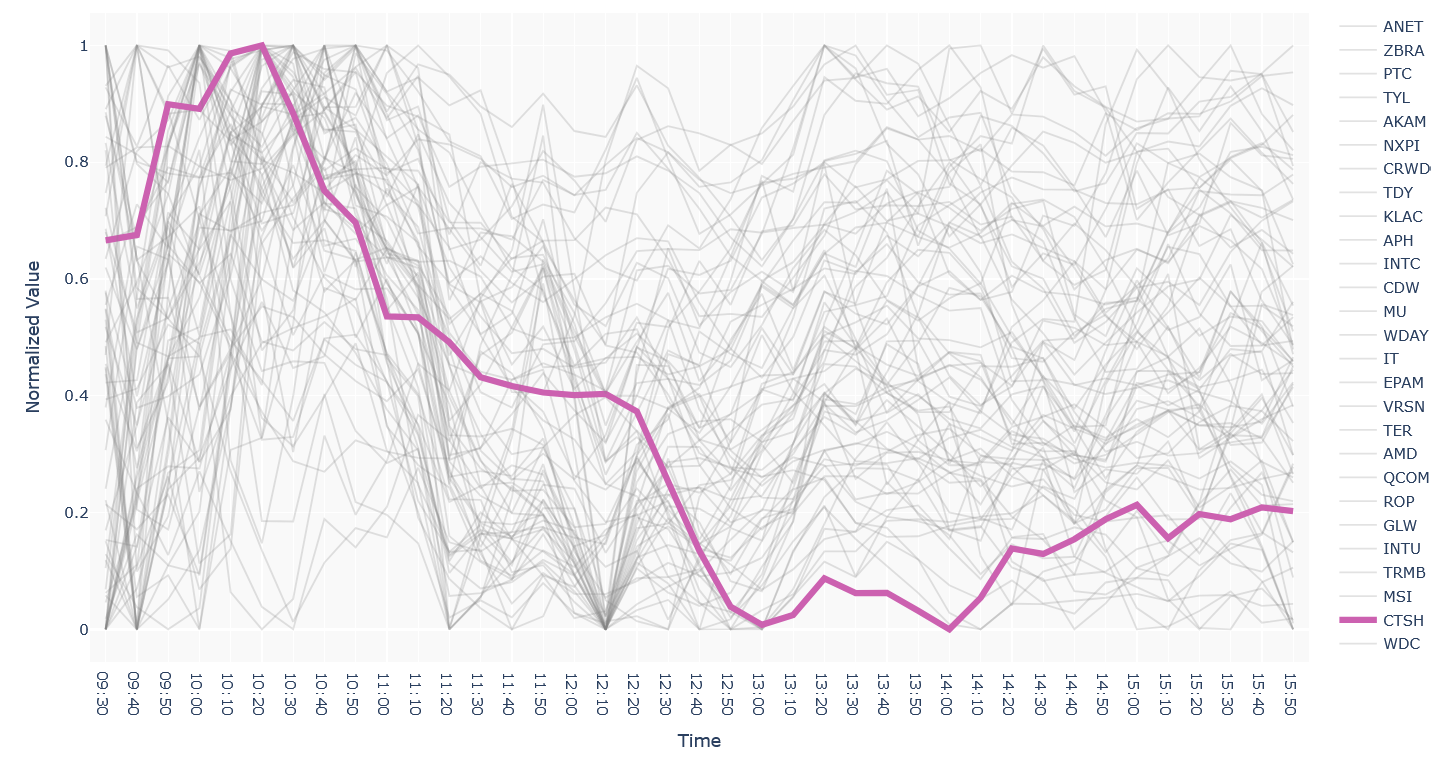
\includegraphics[width=0.4\textwidth]{2D-chart.png}
\caption{Highlighting in 2D line chart.}
\label{fig_2d_dashboard}
\end{figure}

\subsection{Visual Clarity of Highlighting}\label{sec_visual_clarity}
The implementation of the 2D multivariate line graph and the 3D time series projection provided significant observational advantages. In the 2D view, as shown in Figure \ref{fig_2d_dashboard}, the dynamic highlight feature successfully allowed users to select a single asset track or multiple tracks simultaneously. When this feature was activated, the selected trajectories maintained their distinct high contrast color coding while the unhighlighted time series were rendered in a uniform grey color. Observations confirmed that this visual reduction eliminated occlusion for the primary targets while still preserving the necessary contextual background to evaluate broader market correlations. When analyzing denser subsets, the 3D projection mapped distinct instruments along the Y axis. Observations confirm that this spatial separation transformed the traditional hairball effect into independent parallel lines, which is captured in Figure \ref{fig_3d_projection}.

\begin{figure}[h]
\centering
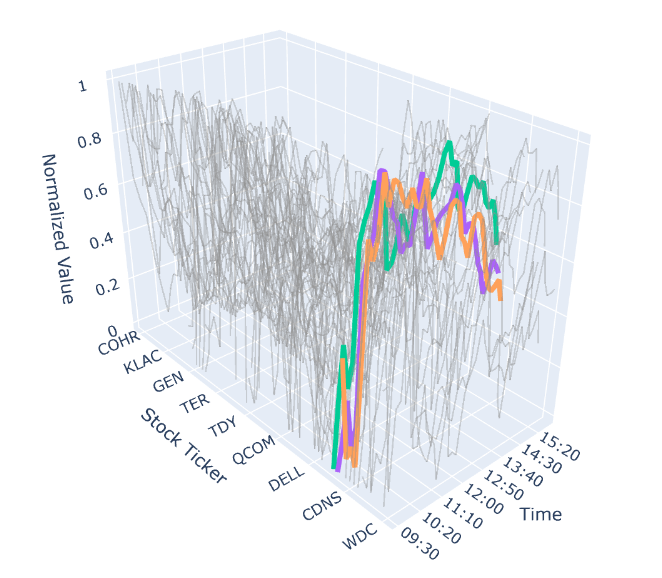
\includegraphics[width=0.4\textwidth]{3D-Plot-highlight.png}
\caption{Highlighting in 3D time series visualization.}
\label{fig_3d_projection}
\end{figure}

\subsection{Spatial separation via Horizon Charts and Sparklines}\label{sec_high_density_results}
The implementation of horizon charts and sparklines enabled the simultaneous vertical stacking of hundreds of assets within a highly compressed visual footprint. Observations of the horizon chart component, as illustrated in Figure \ref{fig_horizon_charts}, confirmed that dividing the continuous data into a five band layered structure successfully preserved the visibility of fine grained price movements. Positive market deviations were rendered using a graduated blue color scale, while negative variations were mirrored and overlaid using a corresponding red color scale. This arrangement allowed high magnitude spikes to remain fully visible within a single narrow row allocation without causing any line crossing artifacts.

\begin{figure}[h]
\centering
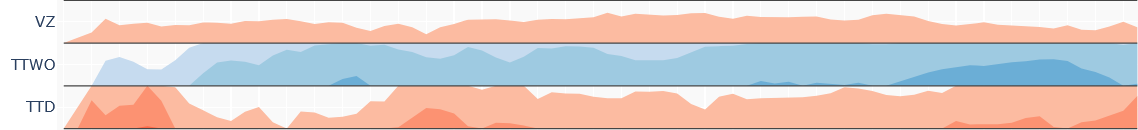
\includegraphics[width=0.4\textwidth]{Horizonchart.png}
\caption{Horizon chart visualization of time series.}
\label{fig_horizon_charts}
\end{figure}

Concurrently, the sparkline component displayed in Figure \ref{fig_sparklines} successfully provided a rapid qualitative summary of historical trends across the entire asset collection. The rendering interface utilized dedicated blue fills for positive values and red fills for negative deviations, anchored by a continuous faint grey baseline for each row. This structural anchor maintained the visual alignment of individual instruments during scanning operations. Furthermore, the inclusion of explicit data gap handling prevented the system from performing erroneous line interpolations across periods with missing data entries. The resulting layout preserved the overall structural patterns of the market while operating under extreme screen space constraints.

\begin{figure}[h]
\centering
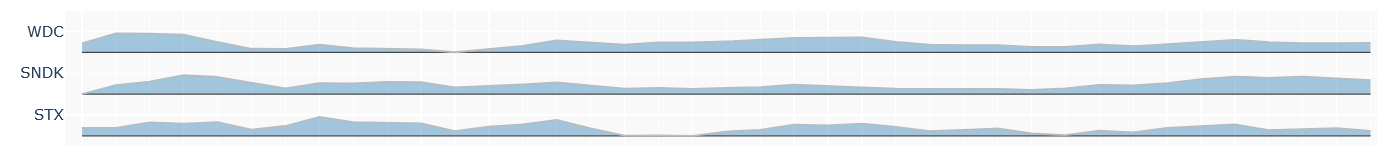
\includegraphics[width=0.4\textwidth]{spartline.png}
\caption{Sparkline visualization of time series.}
\label{fig_sparklines}
\end{figure}

\subsection{Correlation Matrix and Correlation Sorted Heatmap Visualizations}\label{sec_heatmap_results}
The standard pairwise correlation matrix serves as a basic baseline visualization in traditional financial analysis. While it provides a fundamental overview of statistical dependencies, initial evaluation demonstrated severe scalability limitations when analyzing multiple high frequency series simultaneously, as the pairwise matrix expanded quadratically and produced a dense grid of pixelated cells that completely obscured macro level patterns. To address temporal dynamics, a time series heatmap was already implemented in the previous work, mapping selected metrics over time along the X axis and stacking individual instruments along the Y axis.

However, observations during the current development phase confirmed that integrating the automatic correlation sorting pipeline with this existing heatmap makes the visual output significantly more meaningful. Rather than rendering a disordered mix of raw rows, the hierarchical clustering algorithm successfully rearranges the Y axis so that assets with similar temporal behaviors are placed adjacent to one another. This sorting mechanism transforms the visual noise into distinct color blocks and continuous vertical bands of intensity.. Consequently, the updated heatmap design allows analysts to immediately verify co movements and localized volatility spikes that were previously obscured in both the basic baseline matrix and the unsorted temporal layout.

\subsection{Dimensionality Reduction and Cluster Formation}\label{sec_dimensionality_results}
The application of t-SNE and UMAP algorithms provided a spatial visualization of asset dependencies by compressing high dimensional correlation profiles into two dimensional scatter layouts. Observations indicated that the two algorithms produced distinct structural distributions of the asset point clouds. The t-SNE projection, as displayed in Figure \ref{fig_tsne_projection}, successfully isolated highly dense localized clusters of synchronous instruments, although it required greater computational time during real time updates. Conversely, the UMAP implementation generated tightly grouped spatial structures while maintaining global topology relationships across the market segments. In both projections, strongly correlated instruments were mapped in close spatial proximity, transforming abstract statistical dependencies into distinct visual clusters that allowed for immediate identification of parallel market behaviors.

\begin{figure}[h]
\centering
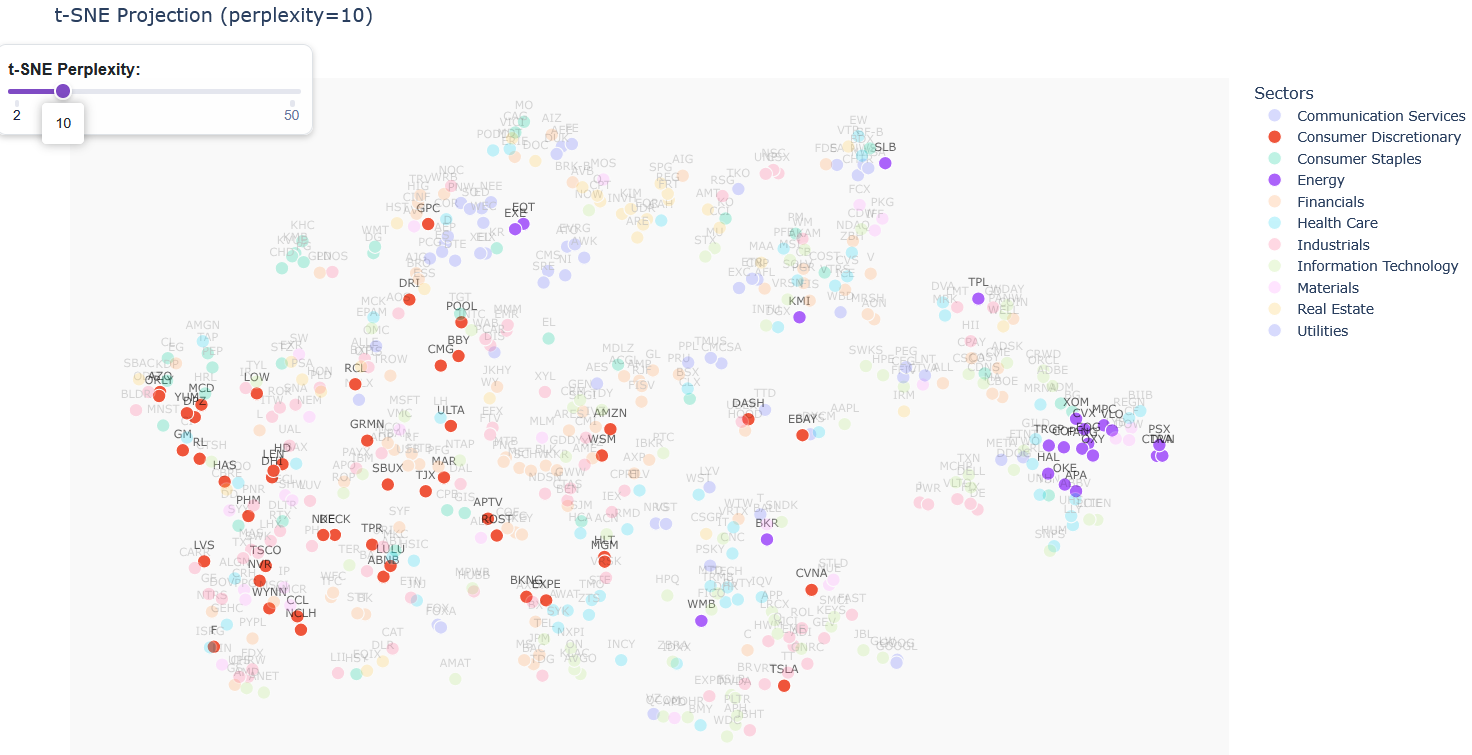
\includegraphics[width=0.49\textwidth]{t-SNE.png}
\caption{t-SNE projection in 2D space.}
\label{fig_tsne_projection}
\end{figure}

\subsection{Impact of Hierarchical Clustering and Filtering}\label{sec_filtering_results}
The implementation of the multi selection dropdown combined with the hierarchical clustering algorithm delivered distinct data reduction advantages. Observations confirmed that the interface allowed users to rapidly alter the density of the macro level visualizations while maintaining strict structural order. When a user selected a targeted subset of assets, the backend callback successfully calculated the real time correlations and executed the sorting pipeline. Rather than displaying uncorrelated assets in a scattered layout, the hierarchical clustering algorithm grouped instruments with identical temporal movements adjacent to one another on the visual canvas. In addition to the global clustering approach, users could activate a reference-based sorting mode by selecting a single instrument as an anchor. In this configuration, all remaining time series were reordered according to their individual Pearson correlation coefficient relative to the chosen reference, placing the most synchronous assets at the top of the visual layout. This targeted sorting mechanism proved particularly effective when analysts sought to confirm whether a specific suspicious instrument was accompanied by a broader group of co-moving assets.  This automatic reorganization transformed the visual noise into clear clustered blocks of activity, enabling the immediate detection of synchronized market trends within the user selected focus area.

\section{Future Work}\label{sec_future_work}
Although the current implementation successfully resolves key visual clutter issues, several technical and functional enhancements remain for future development. The primary technical limitation involves performance degradation when the interface processes an exceptionally high number of concurrent time series. Under dense data loads, the frontend rendering pipeline experiences noticeable latency and lagging during interactive updates. Future work will focus on optimizing the data transfer mechanisms and implementing hardware accelerated rendering solutions to ensure smooth interaction regardless of the dataset volume.

Another significant avenue for exploration is the integration of categorical clustering and group aggregation. Future iterations of the system will introduce a feature allowing analysts to merge individual time series based on predefined market sectors or instrument categories. By checking a dedicated control option, users will be able to collapse a whole group of related assets into a single representative aggregate time series. The entire category will then be evaluated as a single unified vector, dramatically lowering visual complexity and waves of data congestion, allowing for efficient macro level market comparisons before drilling down into individual instruments.

\section{Conclusion}\label{sec:conclusion}

The interactive visual analytics framework developed in this research successfully resolves the challenge of identifying and isolating positively correlated high frequency time series across thousands of financial instruments within specific time windows. By transforming abstract statistical dependencies into structured spatial arrangements, the system completely replaces traditional static layouts with an integrated correlation routing pipeline.
While the original temporal heatmap configuration was already highly effective at displaying correlation patterns, this research significantly improves its analytical utility by integrating the automatic sorting mechanism. The architecture computes pairwise Pearson correlation coefficients across massive data streams and applies a hierarchical clustering algorithm with ward linkage to optimize row ordering. When projected onto the temporal heatmap and high density horizon charts, this sorting pipeline automatically groups assets with synchronized behaviors adjacent to one another along the Y axis. This structural reorganization converts visual noise into distinct color blocks and continuous vertical bands of intensity, allowing analysts to immediately spot co movements and synchronized volatility spikes that were previously fragmented.
Furthermore, the framework externalizes these asset correlations through advanced dimensionality reduction techniques. Compressing high dimensional correlation profiles into two dimensional coordinates via t-SNE and UMAP maps statistical similarity directly onto spatial proximity. In these projections, positively correlated instruments naturally aggregate into dense localized point clouds, providing an instant visual topology of interdependent market sectors. These abstract spatial clusters are seamlessly linked to detailed verification tools, where interactive 2D and 3D line projections enable analysts to isolate specific trajectories using multi track high contrast highlighting. Ultimately, this integration of algorithmic sorting and spatial clustering establishes a scalable solution for validating cross asset dependencies within complex financial environments. In direct response to the primary research question, the framework demonstrates that thousands of high-frequency time series can be efficiently scanned, filtered, and visualized to reliably surface those exhibiting positive correlation within any user-defined time window, making previously hidden market synchronizations immediately accessible to analysts.



%%\section*{References}
%%%%%%%%%% Insert bibliography here %%%%%%%%%%%%%%

%% The Appendices part is started with the command \appendix;
%% appendix sections are then done as normal sections
%% \appendix

%% \section{}
%% \label{}

%% References
%%
%% Following citation commands can be used in the body text:
%% Usage of \cite is as follows:
%%   \cite{key}         ==>>  [#]
%%   \cite[chap. 2]{key} ==>>  [#, chap. 2]
%%   \citet{key}         ==>>  Author [#]

%% References with bibTeX database:

\bibliographystyle{elsarticle-num-names}
\bibliography{BibTexReferences}

\end{document}